\documentclass[iop,apj,tighten]{emulateapj}
%\pdfoutput=1 %for arxiv submission to use pdf
\usepackage{apjfonts} %If missing fonts, comment out this or google apjfonts to download
\usepackage{amsmath,amstext}
\usepackage[breaklinks,colorlinks,citecolor=blue,linkcolor=magenta]{hyperref} 
\usepackage[all]{hypcap} %Links go to figures. This breaks deluxetables; use \capstartfalse \capstarttrue around deluxetables to fix it.

\renewcommand*{\sectionautorefname}{Section} %for \autoref
\renewcommand*{\subsectionautorefname}{Section} %for \autoref

\shorttitle{Galaxy Zoo: Illustris}
\shortauthors{Willett et al.}

\begin{document}

\title{Crowdsourced morphological classifications of Illustris synthetic galaxy images}
\author{K.W. Willett\altaffilmark{1} et al.}
\affil{$^1$University of Minnesota}

\begin{abstract}
Abstract.
\end{abstract}

\keywords{keywords}
\maketitle

\section{Science case}

Crowdsourced classifications of Illustris synthetic images \citep{sny15,tor15} using the Galaxy Zoo \citep{lin08,wil13} interface. 

\section{Data}

\subsection{Image creation}\label{ssec:image_creation}

The majority of the details for the mock stellar image creation are given in \citet{tor15} and \citet{sny15}. 

For Galaxy Zoo, the individual pixel values of the \textsc{SUNRISE} \citep{jon06a,jon10} output and SDSS mosaics were added together in the same units after correctly matching the pixel sizes.  No other noise scalings or additional shot noise were introduced. Foreground and background objects in the SDSS images are treated identically, since the lack of accurate distances for all objects makes it impossible to place them at the correct ``depth'' with respect to overlapping sources. 

The positions of the backgrounds are ``semi-random'' within a large SDSS field centered at $\alpha=XX.XXX,\delta=YY.YYY$ and a size of $\sim ZZ$~deg$^2$. We added a simple procedure to avoid positioning bright stars and other artifacts near the centers of the cutouts. 

\subsection{Galaxy Zoo classification}
As of 15 Feb 2016, there have been 17,046 images classified in GZ-Illustris. 

The total Illustris sample has 110,256 images. That's from 6,891 unique galaxies using a mass-limited sample from the $z=0$ slice in the Illustris-1 simulation \citep{vog14a}. Each galaxy has 16 corresponding composite images --- 1~galaxy $\times$ 4~camera angles $\times$ 4~randomly-selected backgrounds. The total set of images is split into three groups:

\begin{itemize}

\item {\tt fixed\_mass} (10,832~galaxies) --- I selected two narrow mass ranges (low and high) and then selected images with all camera angles and backgrounds within it. This is for analyzing the effect of viewing angle and background on morphological accuracy.
\item {\tt fixed\_view} (6,214~galaxies) --- these span the full mass range of the sample, but with only 1~camera angle and background per galaxy. This is for doing an initial survey of the morphological distributions. The reason that this isn't 6,891 is because several hundred of the images were already classified in {\tt fixed\_mass}.
\item {\tt full\_sample} (93,210~galaxies) --- all the rest.

\end{itemize}


Both the {\tt fixed\_view} and {\tt fixed\_mass} samples were completed by Feb~2016 at 40~classifications each. GZ-Illustris is now paused, so the {\tt full\_sample} doesn't have any classifications yet. 

\section{Analysis}

Figure~\ref{fig:piechart} shows a summary of the morphological demographics for the entire sample. 

\begin{figure*}
\centering
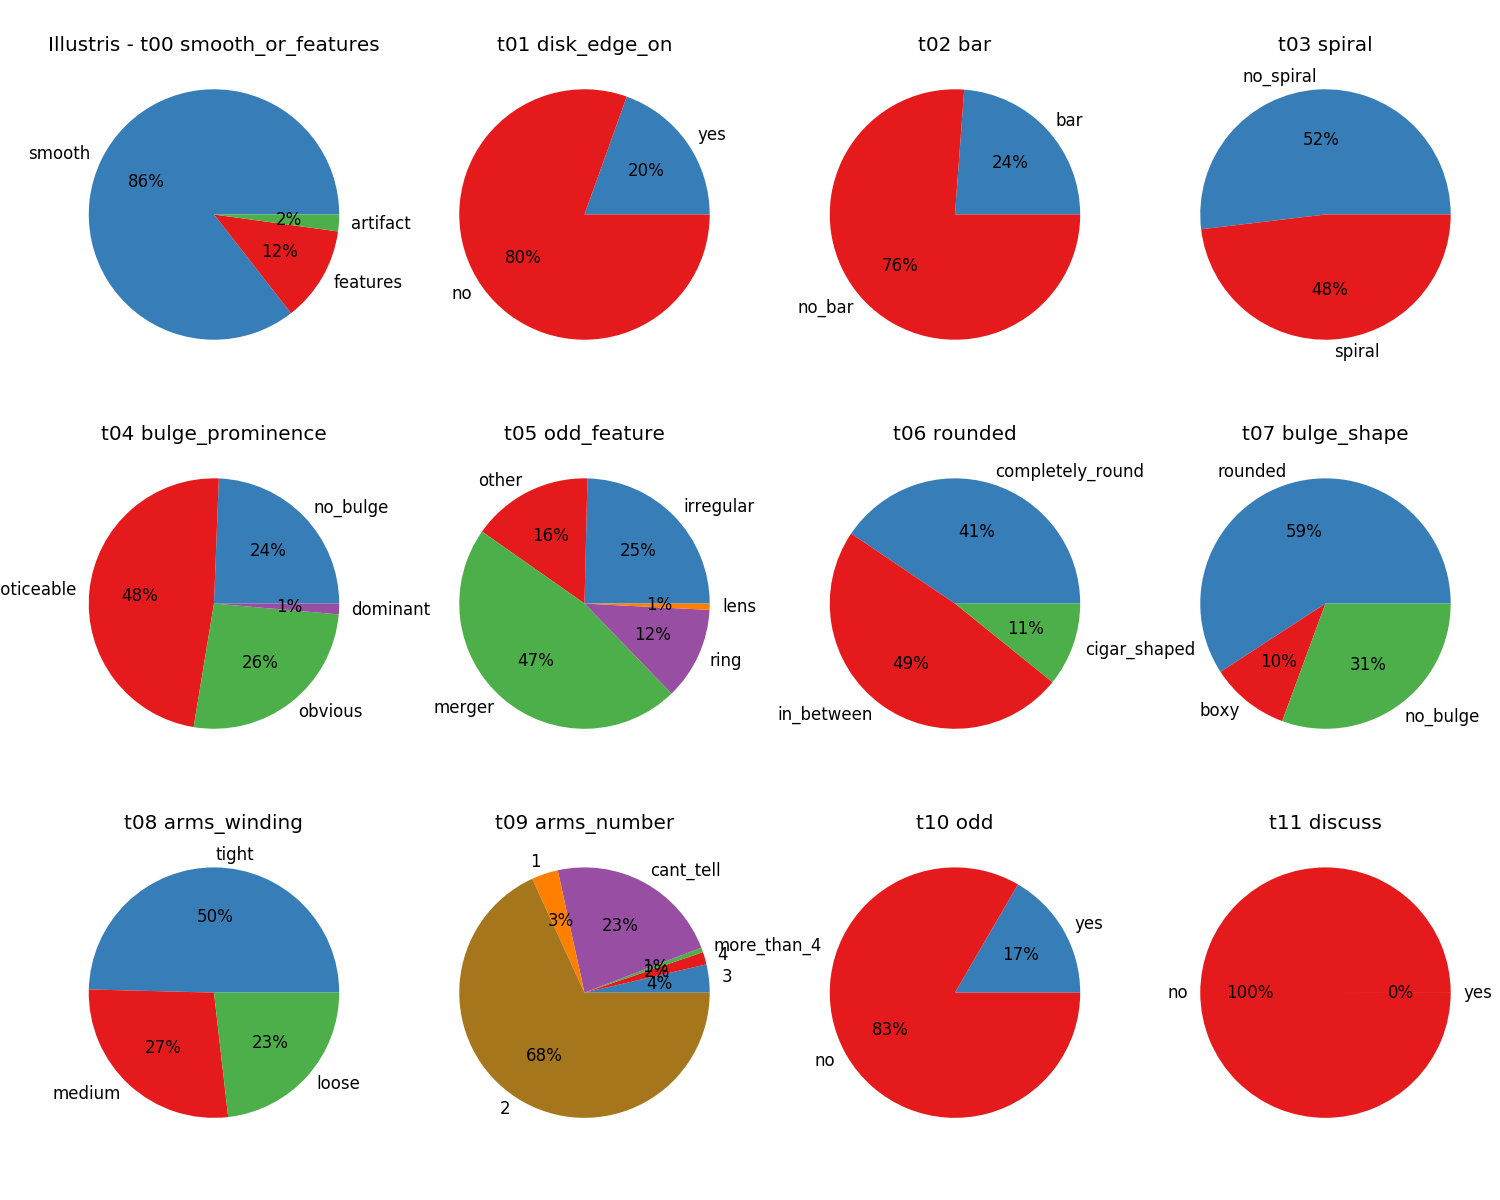
\includegraphics[width=160mm]{../plots/pie_illustris.png}
\caption{Distribution of the plurality morphological category for each task in GZ:Illustris. Labels show the percentage of each morphology only for those galaxies for which the question was reached in the hierarchical tree.\label{fig:piechart}}
\end{figure*}


\acknowledgments{
}

\bibliographystyle{yahapj}
\bibliography{kwrefs}

\end{document}
